%% 多分タイトルとか主張が明確でないのが問題。
%% FDPS の改良を、

%% ・リング系向けのもの
%% ・大規模並列計算機向けのもの
%% ・ヘテロジニアスメニーコア向けのもの
%% ・B/F 小さいマシン向けのもの
%% ・ネットワークが××なマシン向けのもの
%% ・上記の組み合わせとして発生するもの

%% くらいに分類して整理する必要がある

%% そうすると、タイトル、アブストラクトは、

%% Improvement of parallel efficiency of particle-based simulations on
%% present and near-future large-scale parallel computers




%% Modern large-scale machines are fast
%%   enough to follow the evolution of more than $10^{12}$ particles for
%%   more than $10^4$ orbits. However, existing parallel $N$-body codes
%%   cannot achieve reasonable efficiency on modern machines, and we need
%%   to apply many new algorithms to achieve reasonable efficiency.
%%   New algorithms we developed are (1) The use of same interaction
%%   list over multiple timesteps, (2) The use of the cylindrical coordinate
%%   for the domain decomposition and the tree construction. 3)
%%   Rotation of particles to compensate for the Kepler rotation,
%%   4) Construction of ``super domains'' to eliminate global all-to-all
%%   communications and 5) The use of near-optimal static scheduling
%%   algorithm for distributing interaction calculations to multiple
%%   cores in one process.
   
%%   We have implemented these new algorithms to FDPS (Frame Work for
%%   Developing Particle Simulators) and measured the performance on
%%   Sunway TaihuLight. We achieve 3.83 Pflops, or 31 \% of the
%%   theoretical peak on 16384 processes (4096 nodes), when we use 16G
%%   particles. We plan to use this code for the study of global dynamics
%%   of rings. The generic version of the code is publicly available. 






\documentclass[]{pasj01}
%\documentclass[draft]{pasj01}
%\documentclass[proof]{pasj01}
\draft
%%%%%%%%%%%%%%%%%%%%%%%%%%%%%%%%%%%%%%%%%%%%%%%%%%%%%%%%%%%%%%%%
\usepackage{graphicx}
%\usepackage{listings}
%\usepackage{comment}
\usepackage{color}
\usepackage{booktabs} % For formal tables
\usepackage{bm} % For formal tables
%\usepackage{amsmath}
\newcommand{\myvec}[1]{\vec{#1}}
\newcommand{\redtext}[1]{\textcolor{red}{#1}}
\newcommand{\icarus}{Icarus}
\newcommand{\pasa}{Publications of the Astronomical Society of Australia}
%%%%%%%%%%%%%%%%%%%%%%%%%%%%%%%%%%%%%%%%%%%%%%%%%%%%%%%%%%%%%%%%

\begin{document}

\title{Improvement of parallel efficiency of particle-based simulations on
present and near-future large-scale parallel computers}

\author{Masaki \textsc{Iwasawa}\altaffilmark{1}}
\email{masaki.iwasawa@riken.jp}

\author{Long \textsc{Wang}\altaffilmark{2,1}}
\email{long.wang@riken.jp}

\author{Keigo \textsc{Nitadori}\altaffilmark{1}}
\email{keigo@riken.jp}

\author{Daisuke \textsc{Namekata}\altaffilmark{1}}
\email{daisuke.namekata@riken.jp}

\author{Miyuki \textsc{Tsubouchi}\altaffilmark{1}}
\email{miyuki.tsubouchi@riken.jp}

\author{Junichiro \textsc{Makino}\altaffilmark{3,1,4}}
\email{makino@mail.jmlab.jp}

\author{Zhao \textsc{Liu}\altaffilmark{5}}
\email{liuzhao@mail.nsccwx.cn}

\author{Haohuan \textsc{Fu}\altaffilmark{6,5}}
\email{haohuan@tsinghua.edu.cn}

\author{Guangwen \textsc{Yang}\altaffilmark{7,6,5}}
\email{ygw@tsinghua.edu.cn}

\altaffiltext{1}{RIKEN Advanced Institute for Computational Science}

\altaffiltext{2}{Helmholtz Institut f\"{u}r Strahlen und Kernphysik}

\altaffiltext{3}{Department of Planetology, Graduate School of
  Science, Kobe University}

\altaffiltext{4}{Earth-Life Science Institute, Tokyo Institute of
  Technology}

\altaffiltext{5}{National Supercomputing Center in Wuxi}

\altaffiltext{6}{Ministry of Education Key Lab. for Earth System
  Modeling, and Department of Earth System Science, Tsinghua
  University}

\altaffiltext{7}{Department of Computer Science and Technology,
  Tsinghua University}

\KeyWords{Methods: numerical --- Galaxy: evolution --- Cosmology: dark
  matter --- Planets and satellites: formation}

\maketitle

\begin{abstract}

 In this paper, we describe several new algorithms we developed for
 large-scale particle-based simulations on  present and near-future
 large-scale HPC systems. It has become more and more difficult to
 achieve high efficiency on many of  numerical simulations on modern
 HPC systems, for a variety of reasons. We can summarize the reasons as
 (a) very large number of computing cores, exceeding $10^7$ on recent
 machines, (b) relatively low main memory bandwidth , (c) even lower
 network bandwidth, and in some cases (d) communication bottleneck
 between general-purpose CPUs and ``accelerator''. Historically,
 the efficiency achieved with $N$-body simulations on high-end HPC
 systems has been pretty high, such as more than 50\% of the
 theoretical peak speed. However, on some of precent or planned
 architecture, even the best parallel implementation, after careful
 performance tuning, would achieve less than 5\%.
 In this paper, we analyse the reason for such low efficiency and
 propose a combination of new algorithms designed to improve the
 performance of $N$-body simulations on modern HPC systems.
 New algorithms can be divided into three categories. Algorithms of
 the first category are designed to reduce the calculation cost of the
 part other than the pure interaction calculation. Those in the second
 category are  designed to reduce communication between processes, and
 those in the third category are optimization specific to the geometry
 of the physical system. 
  
  We have implemented these new algorithms to FDPS (Framework for
  Developing Particle Simulators) and measured the performance on
  Sunway TaihuLight. We achieve 3.83 Pflops, or 31 \% of the
  theoretical peak on 16384 processes (4096 nodes), when we use 16G
  particles. We plan to use this code for the study of global dynamics
  of rings. The generic version of the code is publicly available. 
  
\end{abstract}

\section{Introduction}
\label{sect:intro}

In this paper, we describe the new algorithms we implented to FDPS
(Framework for   Developing Particle Simulators, [ref here]). FDPS is
designed to make it easy for many researchers to develop his/her own
programs for particle-based simulations. To develop efficient parallel
programs for particle-based simulations requires a very large amount
of work, like the work  of a large team of people for many years. This
is of course true not only for the particle-based simulations, but
practically for any field of computational science. The main reason
is that the modern HPC (high-performance computing) platforms have
become very complex, and thus requires lots of efforts to develop
complex programs to make efficient use of such platforms.

Typical modern HPC systems are actually a cluster of computing nodes
connected through a network, each with typically one or two processor
chips. Largest systems at present consists of around $10^5$ nodes, and
we will see even larger systems soon. This extremely large number of
nodes makes the design of inter-node network very difficult, and the
design of parallel algorithm also becomes very difficult. We need to
make very precise balance for the calculation times of all nodes, and
we need to make the time necessary for communication small enough so
that the use of large systems is meaningful. The communication
bandwidth between nodes is much lower than the main meory bandwidth,
which itself is very small compared to the calculation speed of
CPUs. Thus, it is crucial to avoid communications as much as possible.
It can easily happen that calculation time would show increase,
instead decrease, when we use a large number of nodes.

In addition, the programming environment available on present-day
parallel systems is very poor. What is most widely used if MPI, in
which we need to write the program for a single node, instead of
expressing what should be done for the entire physical system we are
dealing with. We also need to write explicitly how each node
communicate with all others in the system. Just to write and debug the
program is difficult, and it has become nearly impossible for any
single person or even for a group of people to develop large-scale
simulation programs which run efficiently on modern HPC systems.

Moreover, this extremely large number of nodes is just one of the many
serious difficulties in using modern HPC systems, since within one
node, there are many other levels of parallelisms which should be
taken care by programmers. To make the matter even more complicated,
these multiple levels of parallelsm are interwoven with multiple
levels of memory hierarchy with varying bandwith and latency. For
example, the ``post-K'' computer, which is under development in Japan
as of the time of writing, will have 48 CPUs (cores) in one
chip. These 48 cores are divided into four groups, each with 12
cores. Cores in one group share the level-2 cache memory. The cache
meories in different groups communicate with each other through
cache-cohelency protocol. Thus, the access of one core to the data
which happens in its level-2 cache is fast, but that in the cache of
other groups can be very slow. Also, the access to the main memory is
much slower, and that to local level-1 cache is much faster. Thus, we
need to take into account the number of cores and the size and speed
of caches at each level to extract an acceptable performance. To make
the matter words, many of
modern microprocessors have level-3 or even level-4 caches.

As the result of these difficulties, only a small number of reserchers
(or groups of reserchers) can develop their own simulation
programs. In the case of cosmological and galactic  $N$-body and SPH
simulations, Gadget (ref) and  pkdgrav (ref) are most widely used. For
star cluster simulations, NBODY6++ (and NBODY6++GPU) is effctively the
standard. For planetary ring dynamics, REBOUND has been
available. There has been no public code for simulations of planetary
formation process until recently.

This situation is clearly unhealthy. In many cases, the physics need
to be modeled is quite simple: particles interact through
gravity, and with some other interactions such as physical
collisions. Even so, almost all researchers are now forced to use
existing programs  developed by someone else, simply because HPC
platforms have become too difficult to use. To add some  functionality 
which is not already implemented in existing programs can be  very
difficult. 

In order to make it possible for researchers to develop their own
parallel codes for particle-based simulations, we have been developing
FDPS (Framework for Developing Particle Simulators, [ref here]).

The basic idea of FDPS is to separate the code for parallelization and
that for interaction calculation and numerical integration. FDPS
provides the library functions necessary for parallelization, and
using them researchers write programs very similar to what they wiuld
write for single CPU. Parallelization usign MPI and on multiple cores
in single node are taken care of by FDPS.

FDPS provides three sets of functions. One is for the domain
decompositiom.  Given the data of particles on each nodes, FDPS
constructs the decomposition of the computational domain. These
domains are assigned to MPI processes.  The second one is to send
particles to the computing nodes according to their coordinate. Each
particle shuld be sent to tje appropriate MPI process with domain in
which it exists. The third set of functions perform the interaction
calculation. FDPS uses parallel version of Barnes-Hut algorithm, for
both of long-range interactions such as gravtational interactions and
short-range interactions such as intermolecular force or SPH
interaction. Application program gives the function to perform
interaction calculation for two groups of particles (one group
exerting force to another), and FDPS calculates the interaction using
that function.

FDPS offers very good performance on large-scale parallel systems
consisting of ``homogeneous'' multi-core processors, such as K
computer (ref) and Cray systems based on x86 processors. On the other
hand, the architecture of large-scale HPC systems have been shifting
from homogeneous multi-core processors to accelerator-based systems
and heterogeneous multi-core processors.

GPGPUs are most widely used accelerators, and are available on many
large-scale systems. They offer the price-performance ratios and
performance per watt numbers significantly better than those of
homogeneous systems, primarily by integrating a large number of
relatively simple processors on single accelerator chip.  On the other
hand, Accelerator-based systems have two problems. One is that for
many applications, the communication bandwidth between the CPU and the
accelerator becomes the bottleneck. The second one is that because the
CPU and the accelerator have separate memory spaces, the programming
becomes complex and we cannot use existing programs.

Though in general it is difficult to use accelerators, for
particle-based simulations the efficient use of accelerators is not
very difficult, and that fact is the reason why GRAPE families of
accelerators specialized for gravitational $N$-body simulations had
been successful (ref).  GPGPUs also are widely used both for
collisional (ref) and collisionless (ref) gravitational $N$-body
simulations. Thus, it is clearly necessary for FDPS to support
accelerator-based architectures.

Heterogeneous many-core architecture is not yet very popular, but
expected to become popular. In a processor with heterogeneous
many-core architecture, complex and powerful CPU cores and much
simpler accelerator-like cores are integrated.
Heterogeneous many-core architecture ``solves'' the two
main problems of accelerator-based architecture we described above,
since there is no communication bottleneck between CPU cores and
accelerator cores, and they share the same memory space. 

As of March 2018, the fastst supercomputer
in the world, Sunway TaihuLight, is equipped with processors with
heterogeneous many-core architecture, and the fourth, GYOUKOU system,
also equipped with processors with heterogeneous many-core
architecture. 

These systems with heterogeneous architetecture, though in principle
have ``solved'' the problems of accelerator-based systems, in practice
require new approaches to achieve high efficiency. There are several
reasons why new approaches are necessary
\begin{enumerate}

\item The CPU cores are usually relatively weak.
\item The main memory bandwith is low compared to the performance of
  the accelerator cores.
\item The inter-node network is relatively weak.
\item Programming environment is poor or cannot extract the
  performance of hardware.
\end{enumerate}

The first three resons comes simply from the fact that accelerator
cores are much faster than the CPU cores for the same siliocon area
and power consumption. In addition, in order to achieve good
performance, we need to minimize the power and silicon area spent for
CPU cores.  As a result, all other components look slower compared to
accelerator cores. As we stated above, even in the case of homogeneous
manycore systems, main memory and networks are much slower compared to
CPUs. With heterogeneous systems this problem becomes much more
severe.





Recently,  a number of new
findings have been made on the dynamics of the rings of Saturn,
primarily through the  Cassini mission.
Among the new findings, probably  the most
surprising is that the rings show dynamic changes of structures,
possibly including the formation of new satellites. Another example of
truly new findings of the Cassini mission is the vertical structure at
the outer edge of the B ring. (references necessary here)

For some of these new findings, theoretical explanation based on fluid
approximation has been made. However, many of them cannot be explained
by simple fluid models, and more realistic treatment of ring as
collection of particles interacting through both mutual gravity and
physical collisions is necessary.

Planetary rings are usually at the radii around the Roche limit. Thus,
mutual gravity between particles does not easily lead to the formation
of new satellites. However,  spiral waves 
(``wakes'') in very small scales can be formed through self-gravity,
and it  increases the effective
viscosity and enhances the radial transport of the angular
momentum. On the other hand, the actual ring system seems to consist
of very large number of very narrow rings, separated with distinct
gaps. It has been  believed that high-order resonances with small embedded
satellites (so-called moonlets) form these gaps, but this belief lacks
observational/theoretical support.


Very little simulation-based studies have been done to understand
these new findings. The primary reason for this lack is simply that
simulations of such structures must be global simulations including
self gravity of ring particles, which would require very large number
of particles and thus very large amount of computing resources.

Up to now, most of simulations of ring structures have been local
ones, in which a small patch was cut out from the ring and simulated
under the assumption of the local Hill approximation and periodic
boundary condition \citep{WisdomTremaine1988}. \citet{ReinLatter2013}
performed ``Large-scale'' simulation of viscous overstability in
Saturn's rings, using up to 204,178 particles and up to 10,000 orbits
using this local approach. Because very long simulations are
necessary, the number of particles has been small. They used {\tt
  REBOUND} \citep{ReinLiu2012}, an MPI-parallel $N$-body simulation
code. More recently, \citet{Ballouzetal2017} used {\tt
  pkdgrav}\citep{Stadel2001} for simulations with up to 500k
particles.

Compared to the size of local simulations performed so far, the number
of particles necessary for global simulations might seem too
large. However, such large simulations are not beyond the reach of
present-day supercomputers.

We have developed a framework for developing fast and highly scalable
codes for particle-based simulations, FDPS (Framework for Developing
Particle Simulator) \citep{Iwasawaetal2016}. Using FDPS,
\citet{MichikoshiKokubo2017} performed global simulations of rings
with probably the largest number of particles. They used 300M
particles to model two narrow rings of Chariklo and followed the
system for 10 orbital period. The number of particles they used is
already three orders of magnitude larger than what have been used for
global simulations. They have used Cray XC30 at the Center of
Computational Astrophysics, National Astronomical Observatory of
Japan, with the peak speed of 1 Pflops. In order to model fine
structures of Saturn's rings, we need to increase the number of
particles by another three orders of magnitude.

The total calculation cost is roughly proportional to number of
particles multiplied by the number of orbital periods followed, since
the calculation cost per timestep is $O(N \log N)$ when Barnes and Hut
tree algorithm \citep{BarnesHut1986} is used and the number of
timestep required for ring simulations is essentially independent of
the number of particles. Thus, we can conclude that the size of
state-of-the-art simulations of planetary rings is around $3 \times
10^9$ particle-orbits, or around $3 \times 10^{12}$ particle-steps.

We should note that even though the simulations so far done in this
field is relatively small, that does not mean there is no need or
possibilities for larger scale simulations. If we want to model the
global structures of rings, we cannot rely on local treatment. For
example, the effect of resonances with small satellites can only be
studied using global simulations. On the other hand, the number of
particles one needs for global simulations, even for a very narrow
radial range, is very large. For example, consider A ring of Saturn
with the radius of around $1.3\times 10^5\rm km$. The typical radius
of ring particles is 6 m \citep{ZEBKER1985531}, and the optical depth
of the ring is around unity. Thus, we need $10^4$ particles per $\rm
km^2$ or around $10^{12}$ particles for the radial range of 100
km. With this radial range, we can model many of fine features
observed by Cassini directly.

If we could use particles with larger size, we could reduce the number
of particles required significantly. However, that would change the
viscous diffusion timescale of the ring, and thus what would be
observed. Thus, if at all possible, it is desirable to perform
simulations with particle of real physical radius, which would require
at least $10^{16}$ and ideally $10^{19}$ particle-steps.

In other fields of astrophysics, very large simulations have been
performed. For example, \citet{Ishiyama2014} used $4096^3$ particles
to follow the formation and growth of dark matter halos of smallest
scales. This simulation corresponds to $10^{16}$ particle-steps. Part
of this calculation was performed on K computer. The performance of K
computer is $4.0\times 10^{10}$ particle-steps per second on the
entire K computer, or 60,000 particle-step per second per core for a
processor core with the theoretical peak performance of 16 Gflops
\citep{Ishiyamaetal2012}. The efficiency they achieved is 55\% of the
theoretical peak.

\citet{Bedorfetal2014} performed the simulation of Milky Way Galaxy
using $2.42 \times 10^{11}$ particles on large-scale GPGPU
clusters. The achieved performance is 24.77 Pflops on ORNL Titan, and
one timestep took 5.5 seconds. Thus they have achieved the performance
of $4.4 \times 10^{10}$ particle-steps per seconds. The theoretical
peak performance of Titan is 73.2 Pflops in single precision. Thus,
the achieved efficiency is 33.8\%.

The current super computers are powerful enough to perform a realistic
global ring simulation. Thus we are trying to revile the mechanisms of
formation and evolution of ring structures of the Saturn using the
global ring simulation.

As a first step of the investigation of the ring dynamics, we propose
efficient algorithms of global ring simulations and implement them to
FDPS. To develop the algorithms we use Sunway TaihuLight which is the
first ranked on the top 500 list on Nov. 2017. Its processor (SW26010)
is heterogeneous many-core archetecture. However, since our algorithms
are not specialized for heterogeneous manycore archetecture based
system, they are also useful for other manycore archetecture besed
systems or single- or multi-core CPU based systems.

In this paper, we report new efficient algorithms for the global
planetary ring simulations and the measurement of its performance on
Sunway TaihuLight. The paper is organized as follows. In
section~\ref{sec:TaihuLight}, we briefly describe manycore systems,
especially the features of the Sunway TaihuLight system and its
SW26010 processor. In section~\ref{sec:impl0}, we briefly review the
original implementation of FDPS and the problems with the planetary
ring simulation on TaihuLight. In section~\ref{sec:impl1}, we describe
the algorithms we developing. In section~\ref{sec:result}, we present
the measured performance on TaihuLight. In section~\ref{sec:summary},
we summarize the results.

\section{Manycore System}
\label{sec:TaihuLight}

Recently, super computers installing manycore processors, such as
SW26010, GPU (graphics processing unit), Xeon-Phi and PEZY-SC are
widely used in the field of HPC.  For example, in Nov. 2008 only one
manycore system was on the top 500 list, but in Nov. 2017, about 100
systems have manycore processors on the list. Especially, eight
systems in top 10 have manycore processors in Nov. 2017.

One reason of the increase of using manycore porcessors is low power
consumption of manycore processors compared to single- or multi- core
processors. Power consumption of super computers have become a issue
over ten years, in the point of view of running cost and enviromental
protection. Thus manycore systems would become more inportant in the
field of HPC.

Sunway TaihuLight system is one of the manycore systems. It consists
of 40960 nodes, connected by the network with injection bandwidth of
8GB/s per node. The hardware network bandwidth is large enough for our
purpose.

The processor itself consists of four CGs (core groups), each with one
MPE (management processing element) and 64 CPEs (computing processing
elements). Both MPE and CPE are 64-bit RISC cores. MPE has L1 cache
memories for both instructions and data, and also L2 data cache. On
the other hand, each CPE has L1 instruction cache and 64KB of local
data memory. CPEs can communicate with the main memory through DMA.
Each CPE can initiate multiple asynchronous DMA operations. Thus, it
is possible to write the kernel loop so that the computation, DMA read
for the data which will be necessary for the next iteration, and DMA
write operation of the result of the previous iteration all run
concurrently and thus the communication with the main memory is
completely hidden. This capability of explicit control of
communication with main memory is crucial for achieving high
efficiency.

Each core group is connected to 8GB DDR3 DRAM with the theoretical
peak transfer rate of 34GB/s. The processor runs at the clock
frequency of 1.45GHz, and each core (both MPE and CPE) can perform
four double precision FMA operations. Thus, the theoretical peak
performance of one processor is 3016 Gflops and that of one CG is 754
Gflops.

CPEs in one CG are organized into an $8\times 8$ array, and within
each row or column, low-latency, high-bandwidth point-to-point and
broadcast communications are supported.

Operating system runs on MPE, and by default the user program also
runs on MPE. In order to use CPEs, there are two ways. One is to use
an extension of OpenACC designed for SW26010 processor, and the other
is use a lightweight thread library called Athread. Athread is more
difficult to use compared to OpenACC, but allows fine-grained control
of CPEs.

\section{Problems of Original FDPS Implementation on TaihuLight}
\label{sec:impl0}

In this section, we describe the original implementation of FDPS and
problems we would encounter if we use original FDPS on TaihuLight.

The following gives the steps for parallel Barns-Hut tree code when
using FDPS on CPU-based super computer.

\begin{enumerate}

\item Perform domain decomposition by the multisectin method
  \citep{2004PASJ...56..521M}.
  
\item Exchange particles so that particles belong to appropriate
  domains.
  
\item Construct the ``local'' tree structure from particles in the
  domain.

\item Calculate physical quantities of the tree cell of the local tree.

\item Exchange the information necessary for the calculation of
  interaction from other processes [so called local essential tree
    (LET)].
  
\item Construct the ``global'' tree from the collected information.

\item Calculate physical quantities of the tree cell of the global tree.

\item For small group of particles, construct the interaction list
  during traverse the tree. \label{enum:make_list}
  
\item Calculate interactions on the particles from particles in the
  interaction list. \label{enum:calc_force}

\item Repeat steps \ref{enum:make_list} and \ref{enum:calc_force}
  until the calculation of forces on all particles is completed.
  
\item Integrate the orbits of particles.

\item Go back to step 1.
  
\end{enumerate}

For GPUs, FDPS version 2.0 or later also adopt the extension of this
algorithm, in which multiple pairs of particle groups and lists are
constructed and then passed to GPU \citep{Hamadaetal2009}. In this
algorithm, all computations, except for the actual interaction
calculation in the double loop, is done on general-purpose front-end
computer. During the interaction calculation on GPGPUs, the front-end
computer constructs the next interaction lists. Thus we can hide
constructing interaction list.

If we use this algorithms on Sunway TaihuLight, CPEs are used only for
interaction calculations and the other parts are done on
MPEs. However, this algorithm is not sufficient on Sunway
TaihuLight. This is simply because MPE is too slow compared with
CPEs. The execution time for MPE to perform the tree construction and
tree traversal is more than 10 times longer than that for CPEs to do
the interaction calculation, if the efficiency of the interaction
kernel is reasonably high 30-50\%. The same problem would occur even
if we use CPU-GPU heterogeneous systems with the performance ratio of
CPU to GPU is large. \citet{Bedorfetal2014} avoid this problem by
porting all procedures to GPU side. However, even when this approach
is adopted, getting reasonable efficiency turned out to be not easy,
since then the performance of tree construction and tree traversal
would be limited by the bandwidth of the main memory for random
access.  Thus, traditional approach for Barnes-Hut tree algorithm is
not sufficient for manycore processors.

Thus, it is necessary to introduce some new approach to reduce the
calculation (or main memory access) cost of operations other than the
interaction calculation. We adopted the neighbor-list method used in
molecular-dynamics simulations with short-range interactions, in which
the list constructed before is persistently used for multiple steps
(hereafter we call this method persistent-list method). In next
section, we will describe this method.

\section{New Algorithms for Planetary Ring Simulation on Manycore System}
\label{sec:impl1}

In this section, we describe new algorithms for simulating
self-gravitating planetary ring on manycore system, such as
TaihuLight.

\subsection{Persistent List Method}
\label{subsec:list}

In the global ring simulations, each particle moves on nearly circular
orbit and a logical structure of the tree is almost the same for a
shear time scale of the ring. Thus we can persistently use the same
tree structure and interaction lists for multiple timesteps.

By using the same interaction list persistently, we can reduce the
calculation cost of the part other than the interaction calculation
drastically. While we are using the same interaction list, we skip the
domain decomposition, exchange of particles, construction of the local
tree. We still need to update the physical quantities of the cells of
the local tree, since particles in the lowest level have moved. Then,
using the list of tree cells for the local essential tree, the
communication between the processes is performed. Finally, the
physical quantities of the global tree is updated, and the force
calculation is performed using this updated global tree and the
persistent interaction list.

The steps of persistent list method is as follows.

\begin{enumerate}

\item Perform domain decomposition by the multisection method. \label{enum:1st_step_beg}
  
\item Exchange particles so that particles belong to appropriate
  domains.
  
\item Construct the ``local'' tree structure from particles in the
  domain.

\item Calculate physical quantities of the tree cell of the local
  tree.
  
\item Exchange LETs and memorize them and their destination and source
  processes. \label{enum:LET}
    
\item Construct the ``global'' tree from the collected information.

\item Calculate physical quantities of the tree cell of the global tree.
  
\item For small group of particles, construct the interaction list and
  memorize it during traverse the tree.
  
\item Calculate interactions on the particles from particles in the
  interaction list.

\item Repeat steps 8 and 9 until the calculation of forces on all
  particles is completed.
  
\item Integrate the orbits of particles. \label{enum:1st_step_end}
  
\item Calculate physical quantities of the tree cell of the local tree. \label{enum:other_step_beg}

\item Exchange LETs memorized at step 5.

\item Calculate physical quantities of the tree cell of the global
  tree.

\item Calculate interactions on the particles from particles in the
  interaction list.

\item Integrate the orbits of particles. \label{enum:other_step_end}
    
\item Go back to step \ref{enum:other_step_beg} until the interaction
  list is expired.
    
\item Go back to step \ref{enum:1st_step_beg}.
  
\end{enumerate}

We should note that FDPS memorize not only the interaction list, but
also LETs and their destination and source processes at
step~\ref{enum:LET}. In other words, we can skip the tree traversal
for constructing LETs and the communication of exchanging the number
of LETs among all processes.

\subsection{Tree and Domain Structures on Cylindrical Coordinate}
\label{subsec:cylcoord}

\begin{figure}
  \centering 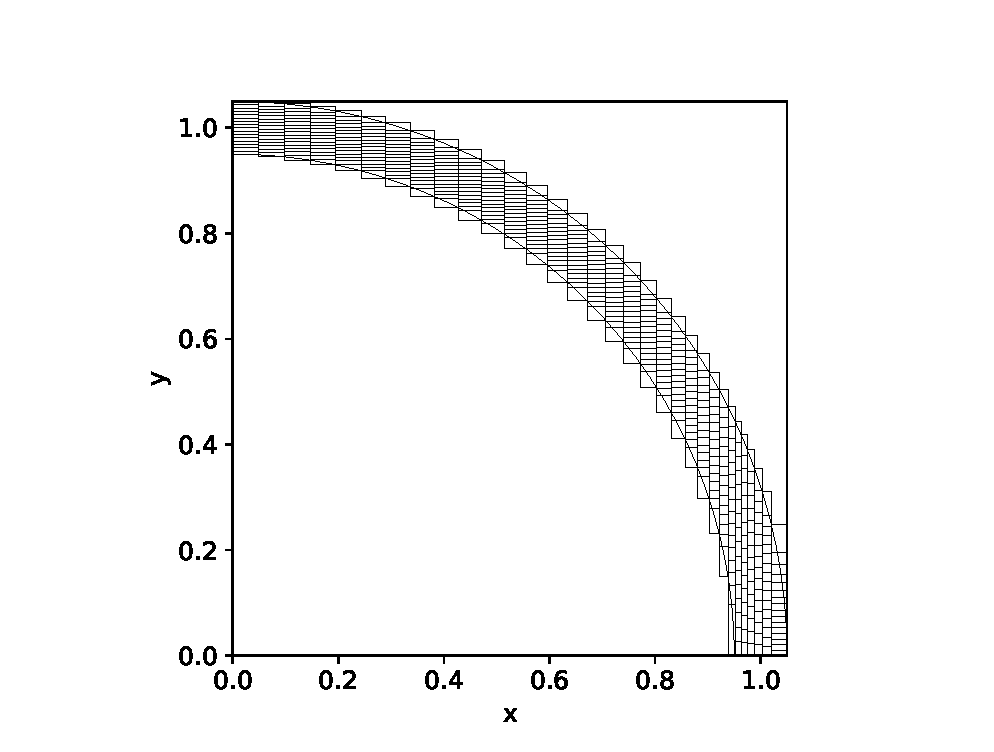
\includegraphics[width=9cm,clip]{./fig/domain_cart.eps}
  \caption{Schematic figure of domain decompostion by the multisection
    method in x-y coordinate. Domains are divided by 32x16.}
  \label{fig:domain_cart}
\end{figure}

\begin{figure}
  \centering
    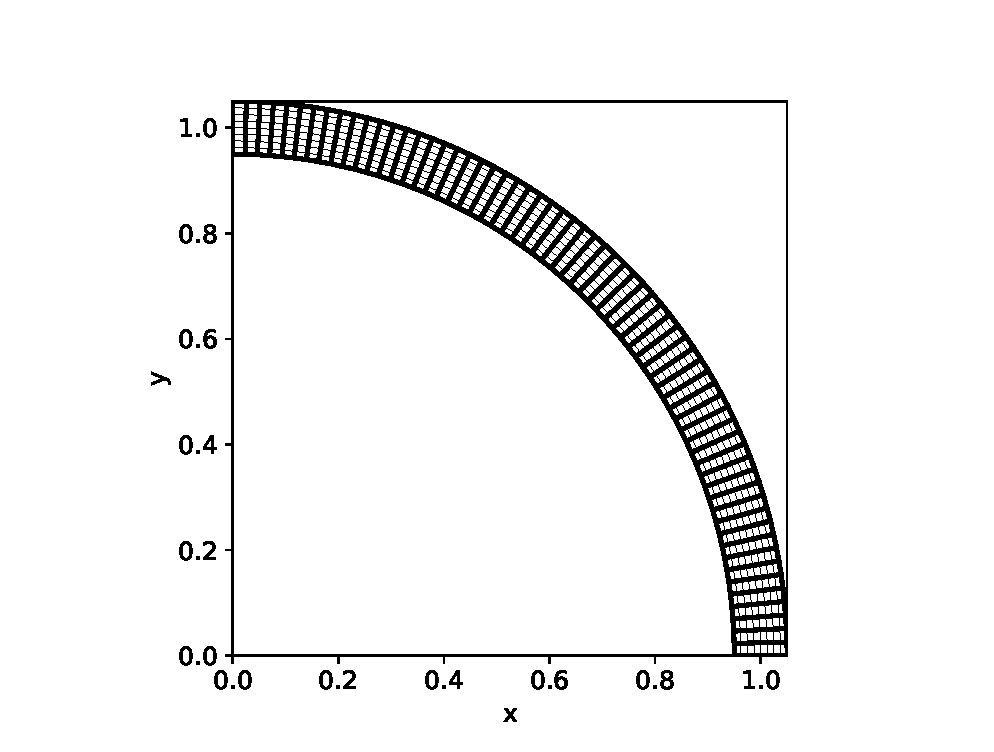
\includegraphics[width=9cm,clip]{./fig/domain_cyl.eps}
  \caption{Schematic figure of domain decompostion by the multisection
    method in cylindrical coordinate. Domains are divided by
    8x64. Large boxes with thick curves indicate super domains (see in
    section \ref{subsec:exlet})}.
  \label{fig:domain_cyl}
\end{figure}

In original implementation, a logical structure of the tree cells and
computational domains are calculated on a Cartesian
coordinate. However, the Cartesian coordinate is not suitable for the
global planetary ring simulations. We can see this reason from
Figure~\ref{fig:domain_cart} which gives an example of domain
decomposition by 32 $\times$ 16 on the Cartesian coordinate for a
quadrant of a ring with the radius of 1.0 and the width of 0.1.

Domains have various shape and some of them have high aspect ratio.
The domains at $x \sim 0$ are elongated along the x direction. On the
other hand, the domains at $x \sim 1$ are elongated along the y
direction. However, the domain shapes at $x \sim 0$ and $x \sim 1$ are
not 90-degree rotation symmetric.

The wide variation of the domain shapes means that tree structure and
the length of the interaction list are the largely different for
different processes. Thus it is difficult to achieve a good load
balance. In addition, the high aspect ratio of the domain increases
the communication costs, because the costs is roughly proportional to
the area of the surface of the domain.

In the point of view of the load balance and communication cost, the
ideal case is that the shapes of all domains are the same
squares. Unfortunately, as long as we use the Cartesian coordinate,
the ideal decomposition is difficult because of the curvature of the
ring.

To approach the ideal domain decomposition, we introduce a cylindrical
coordinate ($r$, $\phi$, $z$). We replace $x$ and $y$ with $\phi$ and
$r$. In this coordinate, a distance between two separate points $ds$
can be approximated by
\begin{equation}
  \label{eq:metric}
  ds^2 = dx^2 + dy^2 + dz^2 \sim d\phi ^2 + dr^2 + dz^2,
\end{equation}
where we assume that the average ring radius is unity.

Figure~\ref{fig:domain_cyl} is the same as
figure~\ref{fig:domain_cart}, but decomposed by 8 $\times$ 64 by using
the cylindrical coordinate. Each domains have almost the same square
shapes. It means the good load balance and the decreasing
communication costs compared to those on the Cartesian coordinate.

We also introduce this coordinate to the tree structure: We evaluate
opening angle of tree cells with the cylindrical coordinate for
constructing the tree, LET and the interaction lists. On the other
hand, for the calculation of the multiple moment of the tree cell and
the interaction calculation, we use the position defined by the
Cartesian coordinate.

For large $\phi$, the approximation of equation~\ref{eq:metric} is
broken and the distance is overestimated. For example, at $\phi=\pi$,
the approximation distance is overestimated by 57 \%. This
approximation means that the accuracy of the force evaluated by
multipole approximation from distant particles is somewhat
worse. However, since the ring system is roughly one-dimensional
structure, the contributions from distant tree cell decreases as
$\phi^{-1}$. Thus our approximation dose not cause serious problem.

\subsection{Counter Rotation of Particles for Exchange Particles}
\label{subsec:exptcl}

Before the construction of the local tree, particles should migrate so
that they belong to appropriate domains. In a reference rest-frame,
the particle move a large distance for multiple timesteps. It means
most particles should go to other domains. It could increase the
communication cost. However, in a rotating frame with the typical
angular speed of the ring, most particles do not seem to move a large
distance. Thus, before the exchange particle, we can reduce the
communication costs by counter-rotating particles by the same angle as
the typical rotation angle of the ring.

\subsection{Super Domain to Remove All-to-All Communication for Exchange LETs}
\label{subsec:exlet}

\begin{figure}
  \centering 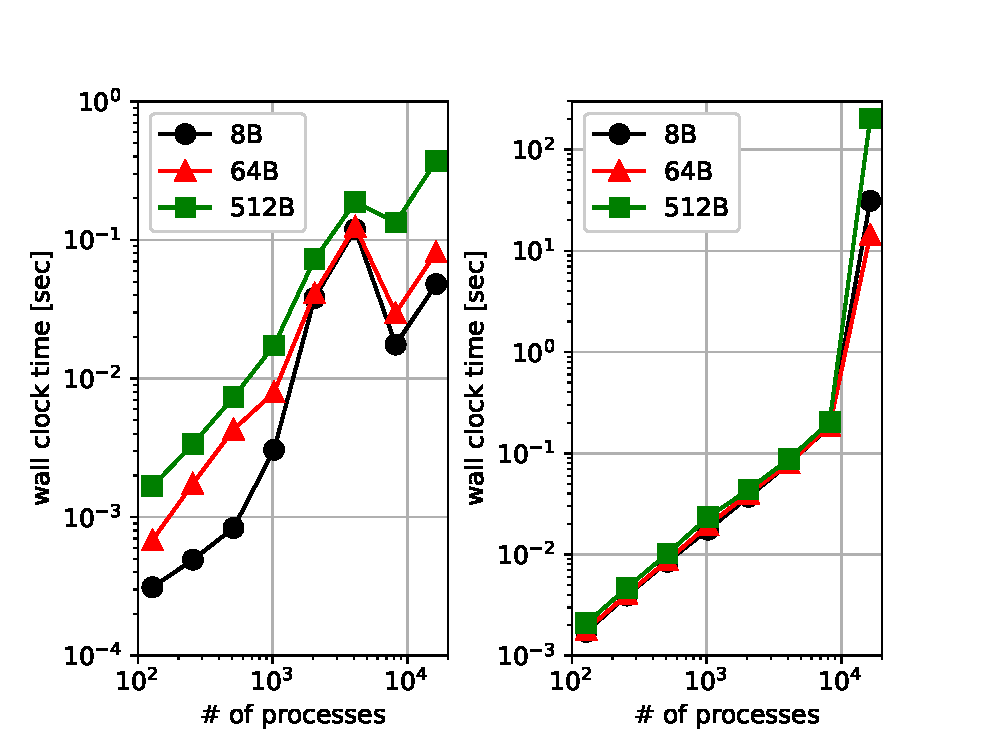
\includegraphics[width=9cm,clip]{./fig/comm_np-wtime.eps}
  \caption{Wall clock time for {\tt MPI\_Alltoall} (left) and {\tt
      MPI\_Alltoallv} (right) against the number of processes.}
  \label{fig:comm_np-wtime}
\end{figure}

\begin{figure}
  \centering
  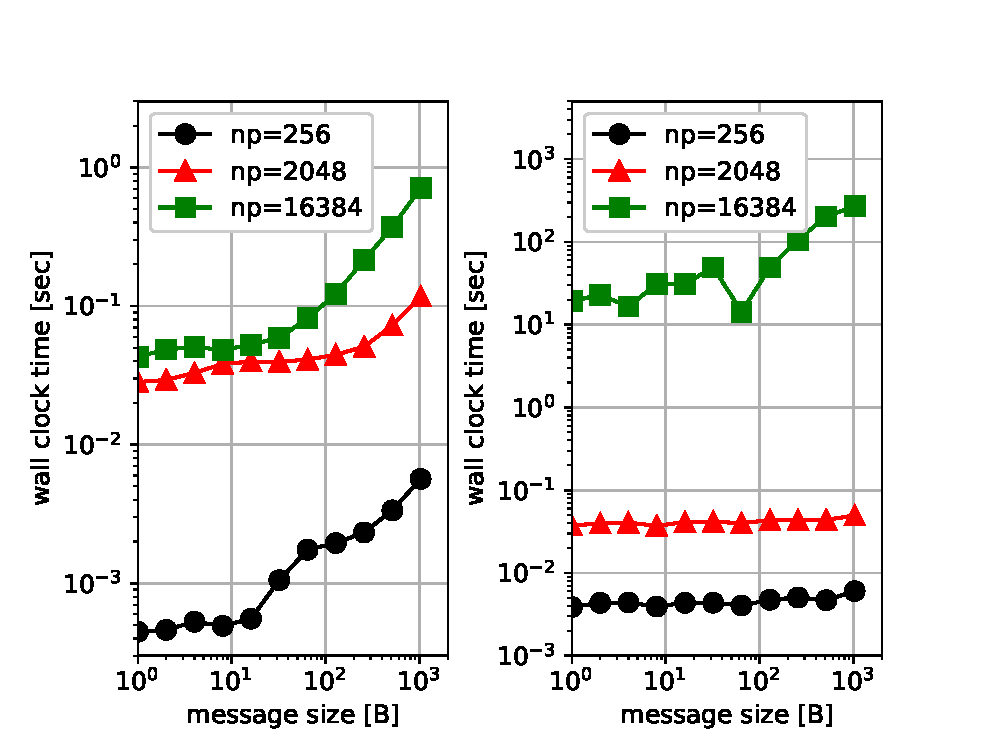
\includegraphics[width=9cm,clip]{./fig/comm_msize-wtime.eps}
  \caption{Wall clock time for {\tt MPI\_Alltoall} (left) and {\tt
      MPI\_Alltoallv} (right) against the size of the message sent per
    process.}
  \label{fig:comm_msize-wtime}
\end{figure}

In the original implementation of the exchange LET, each domain
measure the distances from all other domains and exchange LETs among
all processes. This communication is realized by {\tt
  MPI\_Alltoall(v)}.

Figures~\ref{fig:comm_np-wtime} and \ref{fig:comm_msize-wtime} show
the wall clock times of {\tt MPI\_Alltoall} and {\tt MPI\_Alltoallv}
against the number of processes and the size of the sent message per
process, respectively. The wall clock time is almost linear against
the number of processors for small number of processes. However, for
large number of processes, the time of {\tt MPI\_Alltoallv} rapidly
increase.  From figure~\ref{fig:comm_msize-wtime}, the wall clock time
of {\tt MPI\_Alltoallv} is more than 10 seconds when the number of
processes of 16384 for any message size. As we will see later, the
execution time of our interaction kernel is less than 300 ms, when we
use 1M particles per process. Thus if we use more than $\sim$ 2048
processes, we must avoid to use {\tt MPI\_Alltoallv} (and also {\tt
  MPI\_Alltoall}) .

To avoid all-to-all communications, we introduce a kind of tree
structure to the domains. In principle, if we have the tree of
domains, the all-to-all communication among all processes is not
needed because each process dose not need the multipole moments from
distant domains individually, but only needs locally combined
multipole moment from distant domains.

For simplicity, in our method, we adopt the original domain structure
by the multisection methods as the tree structure with the depth of
two. In other words, the root cell of the domain tree has $n_{\phi}$
sub-cells (hereafter, call it ``super domain''. see
Figure~\ref{fig:domain_cyl}) and each sub-cell (``super domain'') has
$n_{r}$ sub-sub-cells (we do not divide domains in the $z$ direction
because the thickness of the ring is very thin). Here $n_{\phi}$ and
$n_r$ are the number of processes in the $\phi$ and $r$ directions,
respectively.

The steps of the exchange LET using the super domain is as follows.

\begin{enumerate}

\item Each process in a super domain sends the information of its top
  tree cell, such as the multipole moment and the coordinate of the
  cell, to the process with the most inner domain in the same super
  domain (hereafter, call it super process) in r-direction.
   
\item Each super process combines the multipole moment from received
  information.

\item Each super process gathers the combined multipole moments from
  other super domains by using {\tt MPI\_Allgather} in
  $\phi$-direction.

\item Each super process broadcasts the combined multipole moments in
  r-direction. Here, all processes have all other super-domain
  information.

\item Each process measures the distances between own super domain and
  other super domains.

  \begin{description}
    
  \item{(a1)} If the distance is far enough, do nothing because this
    process already received its combined multipole moments at step 3.
  
  \item{(b1)} Otherwise, the process makes LETs for the target super
    domain and sends them to the process with the same process-rank in
    $r$-direction in the target super domain by {\tt MPI\_Isend/recv}.

  \item{(b2)} The process broadcast the received LETs in
    $r$-direction.

  \end{description}
    
\end{enumerate}

If we use this methods, we can completely remove {\tt
  MPI\_Alltoall(v)}.


\subsection{Load Balancer for interaction calculations}
\label{subsec:force}

The interactions are calculated on 64 CPEs in parallel. In our
implementation, different CPEs read different interaction lists and
calculate their interactions. Thus we can avoid reduction of the
forces between CPEs.

To achieve a good load balance, the length of the interaction list on
CPEs should be the same. However, it is difficult to obtain the
optimal solution in a reasonable time. Instead of this, we obtain an
approximated solution by the greedy algorithm. Our implementation is
as follows.

\begin{enumerate}
  
\item Sort the interaction lists by its length (efficient sort
  algorithms on manycore system will be described in appendix 2).

\item Assign the first 64 lists on 64 CPEs, one-by-one.

\item Assign the next interaction list on the CPE with the shortest
  total interaction list.

\item Repeat step 3 until all lists are assigned on CPEs.

\end{enumerate}

Note, at step 3, to find the CPEs with the shortest interaction list,
we use binary tree algorithm.

\section{Performance Results}
\label{sec:result}

In this section, we describe the initial ring model, interaction
model, numerical method and the measured performance of our code.

\subsection{Initial Ring Model}

As an initial model, we make a ring with the radius of 1.0, the width
of 0.01 and the optical depth $\tau$ of 1.0. All particles are
identical and their radii are the same as the Roche radius.  We put
particles on three layers. We put N/3 particles on a regular grid in
the cylindrical coordinate on each layer. The grids are shifted in
both radial and azimuthal by half grid size to the grids on neighbor
layers. The all particles are on circular orbits.

\subsection{Interaction Model}

In our simulations, since $\tau$ is unity, the particles collide with
each other frequently. Since the radius of the particle is the Roche
radius, when the particles collide, the particles rather rebound than
gravitational accreation. To handle this nature of collision, we
regard a particle as a soft sphere. In this model, we consider not
only the gravitational force, but also both a spring and a dashpot
forces. Equation \ref{eq:interaction} gives the definition of the
particle-particle interaction.

\begin{eqnarray}
  \bm F_{ij} = \left \{
  \begin{array}{ll}
     G \frac{m_i m_j}{r_{ij}^3} \bm r_{ij} & \left(r_{ij} > r_{\rm coll} \right) \\
     \left[  G \frac{m_i m_j} {r_{\rm coll}^3} + \frac{m_j}{m_i + m_j} \left( \kappa \frac{ r_{ij} - r_{\rm coll}}{r_{ij}} + \eta \frac{\bm r_{ij} \cdot \bm v_{ij}}{r_{ij}^2} \right) \right] \bm r_{ij} & \left( r_{ij} \le r_{\rm coll} \right)
  \end{array}
  \right.
  \label{eq:interaction} 
\end{eqnarray}

with $\bm r_{ij} = \bm r_j - \bm r_i$, $\bm v_{ij} = \bm v_j - \bm
v_i$, $r_{ij} = \| \bm r_{ij} \|$. Here, ${\mathbf F_{ij}}$ is the
acceleration particle $i$ due to particle $j$, ${\mathbf r_{ij}}$ and
${\mathbf v_{ij}}$ are the relative position and velocity vectors, $G$
is the gravitational constant, $m_i$ is the mass of particle $i$,
$r_{coll}$ is the distance at which two particles collide, and $\eta$
and $\kappa$ are parameters which determine the coefficient of
restitution. We chose these parameters so that the coefficient of
restitution in radial direction is 0.5.

\subsection{Numerical Method}

We use the Barnes-Hut tree method for interaction calculations using
modified FDPS including the algorithms described above. The opening
criterion of the tree $\theta$ is 0.5. The integration method is leap
frog with the shared timestep of $1/128$. We use the same interaction
list for 64 steps.

Over 64 steps, not to miss to detect collisions between particles, we
do not apply multipole approximation to neighboring particles within
three hill radius. To find neighboring particles, we also use the
tree. To do this, each tree cell also have a boundary coordinate
defined by the positions and the radius of particles inside the cell.

In the ring simulation the global structure is not drastically changed
for rotation period. Thus the domain decomposition is done once at the
beginning.

\subsection{Performance}

To measure the performance, we perform both weak-scaling and
strong-scaling tests and measure the time for 64 timesteps. The
execution time is measured by the MPI wallclock timer, and operation
count is from the counted number of interactions
calculated. Particle-particle interaction consists of 9
multiplications, 8 additions, and one square root and one division
operations. Instruction set of Sunway 26010 processor does not include
fast approximation for neither square root or reciprocal square
root. So we implemented fast initial guess and high-order convergence
iteration in software. The number of operations in this part is 7
multiplications, 5 additions and two integer operations. Therefore,
for particle-cell interactions the number of floating-point operations
is 31, and for particle-particle interactions, which include the
repulsive force during physical collisions, is 47. We ignore all
operations other than the interaction calculation, since as far as the
number of floating-point operations is concerned, that for interaction
calculation is more than 99\% of total operation count.

For the weak-scaling measurement, we have performed runs with 1M
particles per MPI process and for the strong-scaling measurement, the
total number of particles is 2G.

\begin{figure}
  \centering
    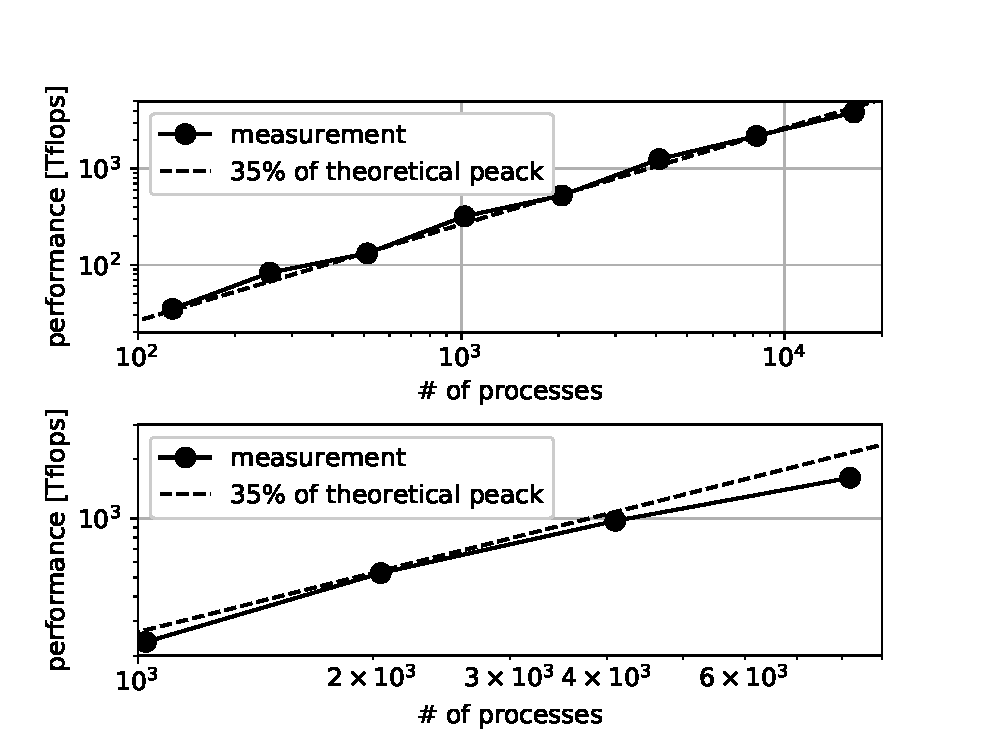
\includegraphics[width=9cm,clip]{./fig/performance.eps}
  \caption{Performance in tera flops for weak-scaling (top) and
    strong-scaling (bottom) tests. The number of particles per process
    is 1M for weak-scaling test. For strong-scaling test, the number
    of particles is 2G. Dashed lines indicate 35 \% of the theoretical
    peak performance of TaihuLight. Closed circles indicate measured
    performance.}
  \label{fig:performance}
\end{figure}

\begin{figure}
  \begin{center}
    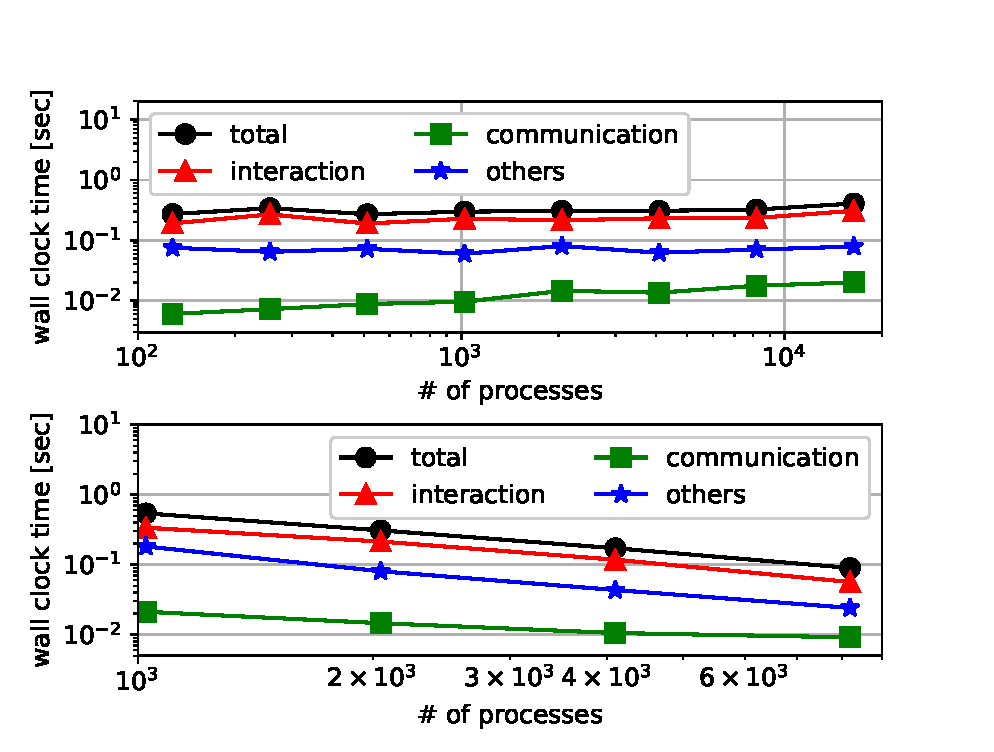
\includegraphics[width=9cm,clip]{./fig/scaling.eps}
  \end{center}
  \caption{Time per timestep for weak-scaling (top) and strong-scaling
    (bottom) tests. The number of particles per process is 1M for
    weak-scaling test. For strong-scaling test, the number of
    particles is 2G.}
  \label{fig:scaling}
\end{figure}

Figure \ref{fig:performance} shows the speed in tera flops, for both
the strong and weak scaling measurements. We can see that the weak
scaling performance is quite good. The performance of run for 16G
particles on 16384 processes (4096 nodes) is 3.83 PFlops, or 31\% of
the theoretical peak performance of the Sunway TaihuLight system. The
strong scaling performance is not perfectly scaled for large number of
processes. However, since our main scientific target is runs with very
large number of particles which has been impossible, weak-scaling
performance is our main interest.

Figure~\ref{fig:scaling} shows the time per one timestep, for both the
strong and weak scaling measurements. The most intensive part is the
interaction calculation. The time for communication increase slower
than linear increase. This is because we removed {\tt
  MPI\_Alltoall(v)} from the communication parts of FDPS (see
Fig. \ref{fig:comm_np-wtime} and \ref{fig:comm_msize-wtime}).

Table~\ref{tab:break_down} shows the breakdown in the case of
weak-scaling test on 8192 processes. The second and the third column
show the time of the first step and the averaged time over 64 steps
for each operation. The forth column shows the values in the second
column divided by those in the third column. Roughly speaking, these
values indicate the speedup factor when we use the persistent list
method.

We find that if we use the persistent list method, the total time
becomes 5.3 times faster.

The ``Local Tree update'' and the ``Global Tree update'' is the time
for updating the physical quantities of the tree cell of the local
tree and the global tree, respectively. These times become slightly
faster. This is because these time include not only the time for
calculating multipole moment of the tree cell, but also the time for
updating tree cell boundaries. However, the tree cell boundaries is
used only for the tree traverse to make interaction lists and
LETs. Thus, we can skip updating boundaries at all steps other than
the first step.

Others mainly include the data copies. The number of data copies also
reduce if we use the persistent list method.

\begin{table}
  \caption{Break down}
  \label{tab:break_down}
  \begin{tabular}{lccc}
    \toprule
    Operation & first step & 64 averaged & speedup\\
    \midrule
    exchange Particles            & 0.308   (18\%)   & 0.00481  (1.5\%)  & 64.0 \\
    Local Tree construction       & 0.0568  (3.3\%)  & 0.000888 (0.27\%) & 64.0 \\
    Local Tree update             & 0.0195  (1.1\%)  & 0.0130   (4.0\%)   & 1.5 \\
    LET construction              & 0.00416 (0.24\%) &  $6.50 \times 10^{-5}$ (0.20\%) & 64.0 \\
    LET communication             & 0.0238  (1.4\%)  & 0.0128  (4.0\%) & 1.86 \\
    Global Tree construction      & 0.178   (10\%)   & 0.0141  (4.4\%) & 12.6 \\
    Global Tree update            & 0.0273  (1.6\%)  & 0.0165  (5.1\%) & 1.65 \\
    Interaction List construction & 0.657   (38\%)   & 0.0103  (3.2\%) & 64.0 \\
    Interaction calculation       & 0.285   (17\%)   & 0.235   (73\%)  & 1.21 \\
    Others                        & 0.150   (8.8\%)  & 0.0156  (4.8\%) & 9.62 \\
    \midrule
    Total                         & 1.71   & 0.323     & 5.29 \\
  \bottomrule
  \end{tabular}
\end{table}

\section{Summary and Discussion}
\label{sec:summary}

\subsection{Real Size Ring Simulation}

As we see in section 1, to investigate the ring structure, we need
$10^{16}-10^{19}$ particle-steps. With our code, we can integrate
about $3.2 \times 10^6$ particles per second per process. In other
words, to investigate planetary ring dynamics, we need $8.7 \times
10^5 - 8.7 \times 10^8$ process hours. If we can use nearly full node
of Sunway TaihuLight or other super computers with similar peak
performance, the simulations would be finished within the reasonable
time. In near future, we will perform these simulations.

\subsection{Extension of Proposed Algorithms}

Proposed algorithms are developed for the planetary ring
simulations. However,we believe that some of them are also useful for
other particle based simulations.

The persistent list method is based on the nature of the ring system
which is the velocity dispersion of the system is very low so that the
particle relative positions keep almost the same for a timestep. Thus
we can use this methods for SPH (Smoothed Particle Hydrodynamics), MD
(Molecular Dynamics) or DEM (Discrete Element Method) simulations.

This method is also useful $N$-body+SPH simulation such as galaxy
formation simulations. This is because the timestep of the simulation
should be determined by SPH particles not by $N$-body particles with
high velocity dispersion.

The super domain method (or introducing tree structure to the domains)
would become necessary to simulate long-range force systems, if we
want to use many processes. This is because the execution time for
all-to-all communication increase at least linearly against the number
of processes.

In this paper, we use only level-two tree structure. This is good
enough for our aim. However, if we use more processes we might need to
introduce more general tree structure to the domain decomposition. We
will study it in near future.

The proposed load balancer for interaction calculations is also useful
on other manycore processors. Since our algorithms is static, in
contrast with a dynamic load balancer, there is no load balancing
overhead during interaction calculation, which would increase as the
number of cores. As an load balancing overhead, our algorithm requires
to sort interaction groups. However, if we use the persistent list
method, the sort is required only at the first step for multiple
steps. In addition, the sort can be parallelized on all cores. Thus
our load balancer could be better compared to other dynamic ones, if
we use the persistent list method on manycore processors.

\subsection{Summary}

In this paper, we described the algorithms and performance of a highly
efficient simulation code for self-gravitating planetary rings on the
Sunway TaihuLight system. We mainly develop five new algorithms: 1)
Persistently use the same interaction list for multiple timesteps. 2)
Use the cylindrical coordinate for constructing the domain and the
tree structure. 3) Counter rotate particles for decreasing
communication costs for exchange particles. 4) Introduce super domains
to remove all-to-all communication for exchange LET. 5) Introduce a
load balancer to assign interaction calculations on cores to achieve a
good load balance.We implement these algorithms to FDPS and we achieve
3.83 PFlops, or 31 \% of the theoretical peak on 16384 processes (4096
nodes). It means we are ready to perform real size ring simulation. In
near future, we will try to perform these simulations to investigate
the formation and evolution of the planetary ring.

\appendix

\section{Force Kernel Tuning on SW21060}

Since the force kernel is the most intensive part in $N$-body
simulation, we need fast force kernel. In our code, different CPEs
calculate different i-particle groups. At first, each CPE stores 256
i-particles and 4 j-particles to its local memory. Then CPE calculate
forces on 256 i-particles from 4 j-particles. To hidden the latency of
reading j-particles, during force calculation, next 4 j-particles are
stored with DMA.

For tuning on the force kernel itself, we develop it in assembly
language because the optimization by the compiler is limited. In
addition, instruction set of Sunway 26010 processor does not include
fast approximation for neither square root or reciprocal square
root. So we implemented fast initial guess and high-order convergence
iteration in software.

\section{Sort on SW21060}

The sorting in the particles frequently used in our code. For example
for the tree construction, we sort the particles by their Morton key.
In original implementation of FDPS, we use the radix sort for integer
numbers. The radix sort is easily parallelized and is known one of the
fastest sort on GPUs.

The bottleneck of the radix sort is the bandwidth of the main memory.
The bandwidth of SW21060 processor is about ten times smaller than
that of the current GPU, such as GTX1080. Thus the radix sort is not
optimal choice on SW21060.

Instead of the radix sort, we used so-called sample-sort method. The
steps of the sample sort is as follows.

\begin{enumerate}
  
\item Sample elements randomly and store them to the local memory.

\item Sort the samples by quick sort on single core.

\item Find the partition to split the sample into 64 segments
  equivalently and assign 64 segments to 64 CPEs one-by-one.

\item Store elements from original array to appropriate local memory.

\item Sort the elements by quick sort on each CPEs.
  
\end{enumerate}

In this method, once we store elements to the local memory, CPEs do
not need to access to the main memory, until the sort is done. Thus
the main memory bandwidth is not serious issue.

\begin{thebibliography}{}

\bibitem[Ballouz et al.(2017)]{Ballouzetal2017} Ballouz, R.-L., Richardson, D.~C., \& Morishima, R.\ 2017, \aj, 153, 146  
  
\bibitem[Barnes \& Hut(1986)]{BarnesHut1986} Barnes, J., \& Hut, P.\ 1986, \nat, 324, 446

\bibitem[B{\'e}dorf et al.(2014)]{Bedorfetal2014} B{\'e}dorf, J., Gaburov, E., Fujii, M.~S., et al.\ 2014, Proceedings of the International Conference for High Performance Computing, Networking, Storage and Analysis, p.~54-65, 54
  
\bibitem[Hamadaetal(2009)]{Hamadaetal2009} Hamada, T., Narumi, T., Yokota, R., Yasuoka, K., Nitadori, K., \& Taiji, M.\ 2009, Proceedings of the Conference on High Performance
  Computing Networking, Storage and Analysis, 62, 12
  
\bibitem[Ishiyama et al.(2012)]{Ishiyamaetal2012}
  Ishiyama,~T., Nitadori,~K., \& Makino, J.\ 2012, Proceedings of the
  International Conference on High Performance Computing, Networking,
  Storage and Analysis, 5, 1
  
\bibitem[Ishiyama(2014)]{Ishiyama2014} Ishiyama, T.\ 2014, \apj, 788, 27

\bibitem[Iwasawa et al.(2016)]{Iwasawaetal2016} Iwasawa, M., Tanikawa, A.,
  Hosono, N., et al.\ 2016, \pasj, 68, 54
  
\bibitem[Makino(2004)]{2004PASJ...56..521M} Makino, J.\ 2004, \pasj, 56, 521
    
\bibitem[Michikoshi \& Kokubo(2017)]{MichikoshiKokubo2017} Michikoshi, S., \& Kokubo, E.\ 2017, \apjl, 837, L13

\bibitem[Portegies Zwart \& B{\'e}dorf(2014)]{PortegiesZwartetal2014} Portegies Zwart, S., \& B{\'e}dorf, J.\ 2014, arXiv:1409.5474
  
\bibitem[Rein \& Latter(2013)]{ReinLatter2013} Rein, H., \& Latter, H.~N.\ 2013, \mnras, 431, 145

\bibitem[Rein \& Liu(2012)]{ReinLiu2012} H. {Rein} \& S.-F. {Liu}, 2012, \aap, 537, 128

\bibitem[Stadel(2001)]{Stadel2001} Stadel, J.~G.\ 2001, Ph.D.~Thesis, 3657
  
\bibitem[Wisdom \& Tremaine(1988)]{WisdomTremaine1988} Wisdom, J., \& Tremaine, S.\ 1988, \aj, 95, 925
  
\bibitem[Zebker et al.(1985)]{ZEBKER1985531} Zebker, H.~A., Marouf, E.~A., \& Tyler, G.~L.\ 1985, \icarus, 64, 531

\end{thebibliography}
  
\end{document}
